% Milestone - Week 1-2 presentation (minimal)
\documentclass[aspectratio=169,10pt]{beamer}
\usetheme{metropolis}
\usepackage{graphicx}

\graphicspath{{../diagrams/}}

\title{Milestone}
\author{Hung Tran}
\institute{Vietnamese-German University}
\date{6 November 2026}

\begin{document}

% ---------------------------------------------------------------- 1. Problem
\begin{frame}{The problem}
A crowdfunding platform holds other people's money for weeks.
Four failures the operator cannot structurally prevent:
\begin{itemize}
  \item \textbf{Custody risk.} Funds sit in the operator's account.
  \item \textbf{Opaque release.} Milestone approval in a private admin panel.
  \item \textbf{Discretionary refunds.} A refund is a support ticket, not a right.
  \item \textbf{Deplatforming.} A campaign and its funds can be removed.
\end{itemize}
Policy fixes raise the cost of misbehaviour. They do not make it impossible.
\end{frame}

% ---------------------------------------------------------------- 2. Solution
\begin{frame}{What the system does}
A creator opens a campaign with a goal, a deadline, and milestones.
Donors contribute native ETH.
\begin{itemize}
  \item Goal missed: any donor withdraws their exact contribution, any time.
  \item Goal met: creator delivers a milestone, posts an evidence hash.
  \item Challenge window opens. No objections: funds release.
  \item Objection quorum reached: milestone disputed, funds freeze.
\end{itemize}
No employee of the platform can move the funds.
\end{frame}

% ---------------------------------------------------------------- 3. Why blockchain
\begin{frame}{Does it need a blockchain?}
The product works on a database. The guarantee does not.
\begin{itemize}
  \item One property requires the chain: donor funds held by code no operator key can redirect.
  \item A database can move money correctly. It cannot make the operator unable to move it wrongly.
  \item The centralised alternative is genuinely good (fast, cheap, refunds work). But every guarantee is a policy, enforceable only after the fact.
\end{itemize}
Where the chain loses: privacy, finality, UX, no fiat, censorship, parameters instead of judgement.
\end{frame}

% ---------------------------------------------------------------- 4. Architecture
\begin{frame}{System architecture}
\centering
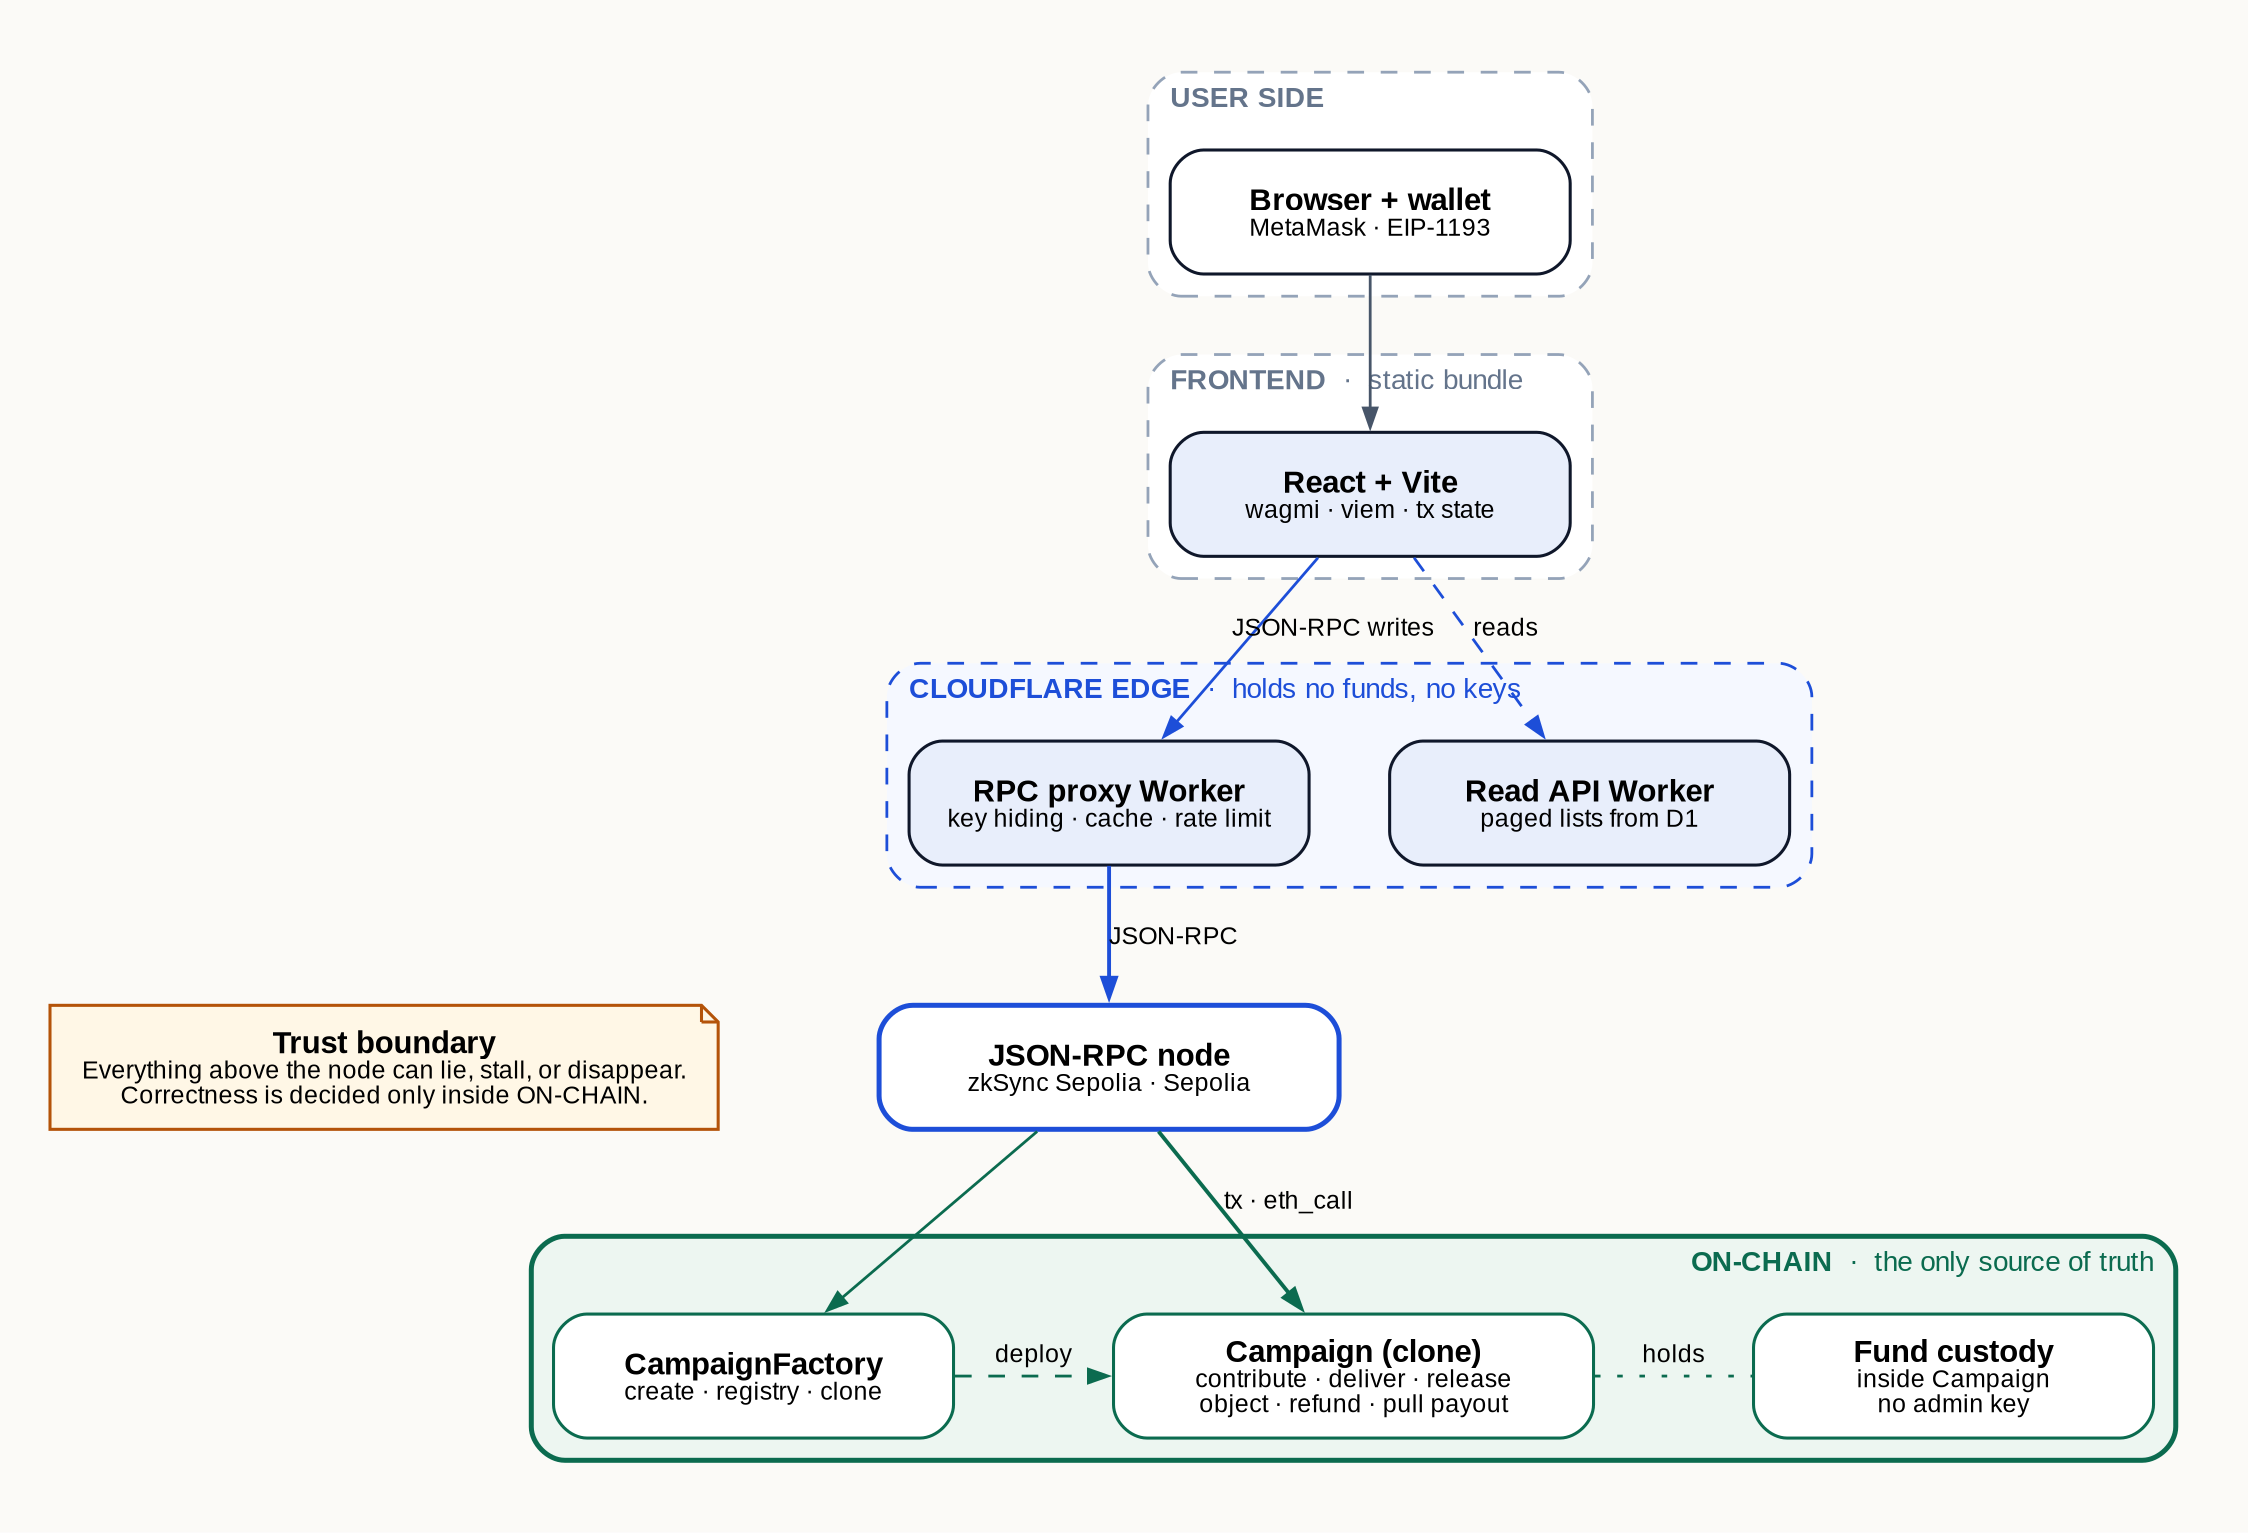
\includegraphics[height=0.55\textheight]{system-architecture-min.png}
\vspace{0.3em}
\small Trust plane (contracts) above, service plane (wallets, RPC, cache, storage, UI) below. The service plane may lie, stall, or vanish. The trust plane is the only source of truth.
\end{frame}

% ---------------------------------------------------------------- 5. Components
\begin{frame}{Components}
\begin{itemize}
  \item \textbf{CampaignFactory:} creates campaigns. Holds no funds.
  \item \textbf{Campaign:} contributions, milestones, payouts, refunds.
  \item \textbf{RPC proxy:} key hiding, caching, rate limiting.
  \item \textbf{Read API:} paged lists from a cache.
  \item \textbf{R2:} files. Integrity via on-chain hash.
  \item \textbf{Turnstile:} anti-spam on create (UI only).
\end{itemize}
Deployment: Anvil locally, zkSync Sepolia for the demo, Ethereum Sepolia as baseline.
\end{frame}

\end{document}
